\documentclass[a4paper]{article}

\usepackage[italian]{babel}
\usepackage[utf8]{inputenc}
\usepackage{graphicx}
\usepackage{amsfonts}
\usepackage{amsmath, amssymb}
\usepackage{parskip}
\usepackage{xcolor}
\usepackage{listings}
\usepackage{colortbl}
\usepackage{hyperref}
\usepackage[a4paper,top=3cm,bottom=3cm,left=2.5cm,right=2.5cm]{geometry}

\definecolor{cell_color1}{RGB}{193, 219, 191}
\definecolor{cell_color2}{RGB}{215, 219, 215}

\lstdefinestyle{mymatlabstyle}{
    language=MATLAB,
    basicstyle=\ttfamily\footnotesize,
    keywordstyle=\color{blue},
    commentstyle=\color[rgb]{0.03, 0.51, 0.16},
    stringstyle=\color{red},
    breaklines=true,
    showstringspaces=false,
    numbers=left,
    numberstyle=\tiny,
    frame=single,
    captionpos=b
}

\lstdefinelanguage{myprocessing}{
    keywords={void, int, float, if, else, for, while},
    sensitive=true,
    comment=[l]{//},
    morecomment=[s]{/*}{*/},
    morestring=[b]",
}

\lstdefinestyle{myprocessingstyle}{
    language=myprocessing,
    basicstyle=\ttfamily\footnotesize,
    keywordstyle=\color{blue},
    commentstyle=\color[rgb]{0.37, 0.37, 0.37},
    stringstyle=\color{red},
    breaklines=true,
    showstringspaces=false,
    numbers=left,
    numberstyle=\tiny,
    frame=single,
    captionpos=b
}

\lstdefinelanguage{myarduino}{
    keywords={void, int, float, if, else, for, while, return, setup, loop, digitalWrite, digitalRead, PROCESSING_ID},
    sensitive=true,
    comment=[l]{//},
    morecomment=[s]{/*}{*/},
    morestring=[b]",
}

\lstdefinestyle{myarduinostyle}{
    language=myarduino,
    basicstyle=\ttfamily\footnotesize,
    keywordstyle=\color[rgb]{0.91, 0.49, 0.09},
    commentstyle=\color[rgb]{0.44, 0.45, 0.45},
    stringstyle=\color[rgb]{0.17, 0.78, 0.75},
    breaklines=true,
    showstringspaces=false,
    numbers=left,
    numberstyle=\tiny,
    frame=single,
    captionpos=b
}


\begin{document}
    
    \begin{figure}
        \centering
        
\includegraphics[width=15cm]{images/Logo.png}
    \end{figure}
    
    \begin{figure}
        \centering
        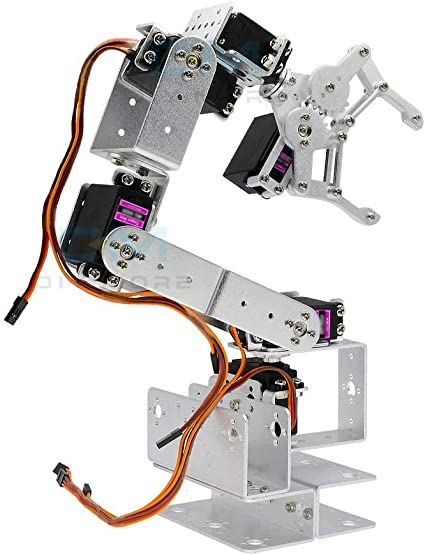
\includegraphics[width=8cm]{images/braccio_robotico.jpg}
    \end{figure}
    
    \title{\textbf{Relazione tirocinio Scorbot}}
    \author{Simone Arcari, matricola: 0292185}
    \date{19/02/2023}
    
    \maketitle
    \newpage
    \tableofcontents
    \newpage
    
    \section{Introduzione}
    
    \begin{text}
        Lo scopo del progetto è quello di controllare la cinematica di un robot di tipo Scorbot mediante simulazione 3D in ambiente Processing con comunicazione seriale tra Processing e la scheda di sviluppo Arduino UNO, che si occuppa del controllo finale degli attuattori utilizzati per la movimentazione dei giunti meccanici. 
    \end{text}
    
    
    \section{Studio del modello matematico}
    
    \begin{text}
        Lo Scorbot utilizzato presenta una struttura leggermente differente da quella solitamente utilizzata in ambito didattico. Inoltre, siccome uno degli obiettivi iniziali era invertire il verso di riferimento degli angoli $\theta_i$, si è reso indispensabile riformulare tutti i passi per il calcolo della cinematica inversa.
    \end{text}
    
    \subsection{Denavit-Hartenberg}
    
    \begin{text}
        Il robot presenta 5 DOF (degree of freedom), è perciò necessario ricorrere al modello di Denavit-Hartenberg per lo studio della geometria dello Scorbot. Per soddisfare l'obiettivo di invertire il verso degli angoli $\theta_i$ sono stati scelti i versi degli assi $z_i$ in direzione opposta rispetto alla rappresentazione degli stessi nella formulazione classica. Effettuati tutti i procedimenti richiesti si giunge alla seguente tabella:\\
    \end{text}
    
    \[
    \begin{tabular}{|c|c|c|c|c|}
        \hline
            \cellcolor{cell_color1} \textbf{i} & \cellcolor{cell_color1} $\mathbf{\theta_i}$ & \cellcolor{cell_color1} $\mathbf{d_i}$ & \cellcolor{cell_color1} $\mathbf{a_i}$ & \cellcolor{cell_color1} $\mathbf{\alpha_i}$\\
        \hline
            \cellcolor{cell_color2} \textbf{1} & $\theta_1^*$ & 0 & 0 & $\Pi/2$\\
        \hline
            \cellcolor{cell_color2} \textbf{2} & $\theta_2^*$ & 0 & $l_2$ & 0\\
        \hline
            \cellcolor{cell_color2} \textbf{3} & $\theta_3^*$ & 0 & $l_3$ & 0\\
        \hline
            \cellcolor{cell_color2} \textbf{4} & $\theta_4^*$ & 0 & $a_4$ & $\Pi/2$\\
        \hline
            \cellcolor{cell_color2} \textbf{5} & $\theta_5^*$ & $d_5$ & 0 & 0\\
        \hline
    \end{tabular}
    \]
    \\
    
    \begin{text}
        Si può osservare che nella tabella figura il parametro $a_4$, ciò è dovuto alla posizione dell'handeffector, che risulta assemblato con una leggera traslazione rispetto all'asse $x_4$. Da ogni riga della tabella si può ora ricavare la matrice del cambio delle coordinate tra $O_{i-1}$ e $O_i$ che indicheremo con $T_{i-1}^i$.
        Questa matrice è nota ed è la seguente:
    \end{text}
    
    \[
    T_{i-1}^i = T_z(\theta_i, d_i)*T_x(\alpha_i, a_i) = 
    \begin{bmatrix}
        cos\theta_i & -sin\theta_i & 0 & 0\\[1ex]
        sin\theta_i & cos\theta_i & 0 & 0\\[1ex]
        0 & 0 & 1 & d_i\\[1ex]
        0 & 0 & 0 & 1\\[1ex]  
    \end{bmatrix}
    *
    \begin{bmatrix}
        1 & 0 & 0 & a_i\\[1ex]
        0 & cos\alpha_i & -sin\alpha_i & 0\\[1ex]
        0 & sin\alpha_i & cos\alpha_i & 0\\[1ex]
        0 & 0 & 0 & 1\\[1ex]  
    \end{bmatrix}
    =
    \]
    
    \[
    = 
    \begin{bmatrix}
        cos\theta_i & -sin\theta_i cos\alpha_i & sin\theta_i sin\alpha_i & a_i cos\theta_i\\[1ex]
        sin\theta_i & cos\theta_i cos\alpha_i & -cos\theta_i sin\alpha_i & a_i sin\theta_i\\[1ex]
        0 & sin\alpha_i & cos\alpha_i & d_i\\[1ex]
        0 & 0 & 0 & 1\\[1ex]  
    \end{bmatrix}
    \]
    \\
    
    \begin{text}
        Si prosegue con il calcolo della matrice del cambiamneto delle coordinate da $O_0$ a $O_5$:
    \end{text}
    
    \[
    T_0^5 = T_0^1*T_1^2*T_2^3*T_3^4*T_4^5 = 
    \begin{bmatrix}
        c_1 c_{234} c_5 + s_1 s_5 & -c_1 c_{234} s_5 + s_1 c_5 & c_1 s_{234} & a_4 c_1 c_{234} + l_3 c_1 c_{23} + l_2 c_1 c_2 + d_5 c_1 s_{234}\\[1ex]
        s_1 c_{234} c_5 - c_1 s_5 & -s_1 c_{234} s_5 - c_1 c_5 & s_1 s_{234} & a_4 s_1 c_{234} + l_3 s_1 c_{23} + l_2 s_1 c_2 + d_5 s_1 s_{234}\\[1ex]
        s_{234} c_5 & -s_{234} s_5 & -c_{234} & a_4 s_{234} + l_3 s_{23} + l_2 s_2 + d_1 - d_5 c_{234}\\[1ex]
        0 & 0 & 0 & 1\\[1ex]  
    \end{bmatrix}
    \]
    
    \begin{text}
        La matrice è stata scritta nella sua forma con notazione compatta dove valgono le seguenti relazioni: \\
    \end{text}
    
    \[c_1 = cos\theta_1, \qquad s_1 = sin\theta_1\]
    \[c_2 = cos\theta_2, \qquad s_2 = sin\theta_2\]
    \[c_5 = cos\theta_5, \qquad s_5 = sin\theta_5\]
    \[c_{23} = cos(\theta_2 + \theta_3), \qquad s_{23} = sin(\theta_2 + \theta_3)\]
    \[c_{234} = cos(\theta_2 + \theta_3 + \theta_4), \qquad s_{234} = sin(\theta_2 + \theta_3 + \theta_4)\]
    
    \subsection{Cinematica diretta}
    
    \begin{text}
        La matrice del cambiamneto delle coordinate $T_0^5$ si compone di una sottomatrice quadrata $R_0^5$, che indica la rotazione di $O_5$ rispetto a $O_0$ e un vettore colonna $\vec{p}$, che indica la traslazione di $O_5$ rispetto a $O_0$. Questa traslazione rappresenta le cordinate dell'handeffector e si ricava nel seguente modo:\\
    \end{text}
    
    \[
    T_0^5*
    \begin{bmatrix}
        0\\[1ex]
        0\\[1ex]
        0\\[1ex]
        1\\[1ex]  
    \end{bmatrix}
    =
    \begin{bmatrix}
        a_4 c_1 c_{234} + l_3 c_1 c_{23} + l_2 c_1 c_2 + d_5 c_1 s_{234}\\[1ex]
        a_4 s_1 c_{234} + l_3 s_1 c_{23} + l_2 s_1 c_2 + d_5 s_1 s_{234}\\[1ex]
        a_4 s_{234} + l_3 s_{23} + l_2 s_2 + d_1 - d_5 c_{234}\\[1ex]
        1\\[1ex]  
    \end{bmatrix}
    \]
    
    \begin{text}
        Solo le prime tre componenti rappresentano le cordinate $[x_d, y_d, z_d]$ , la quarta è superflua. In conclusione la terna di coordinate dell'handeffector rispetto a $O_0$ risulta:
    \end{text}
    
    \[
    \begin{bmatrix}
        x_d\\[1ex]
        y_d\\[1ex]
        z_d\\[1ex]
    \end{bmatrix}
    =
    \begin{bmatrix}
        a_4 c_1 c_{234} + l_3 c_1 c_{23} + l_2 c_1 c_2 + d_5 c_1 s_{234}\\[1ex]
        a_4 s_1 c_{234} + l_3 s_1 c_{23} + l_2 s_1 c_2 + d_5 s_1 s_{234}\\[1ex]
        a_4 s_{234} + l_3 s_{23} + l_2 s_2 + d_1 - d_5 c_{234}\\[1ex] 
    \end{bmatrix}
    \]
    
    \begin{text}
        Dallo studio della struttura del robot ci si rende conto che le coordinate del polso risultano:
    \end{text}
    
    \[
    \begin{bmatrix}
        \textcolor{red}{x_{polso}}\\[1ex]
        \textcolor[rgb]{0.004, 0.5, 0.004}{y_{polso}}\\[1ex]
        \textcolor{blue}{z_{polso}}\\[1ex]
    \end{bmatrix}
    =
    \begin{bmatrix}
        l_3 c_1 c_{23} + l_2 c_1 c_2\\[1ex]
        l_3 s_1 c_{23} + l_2 s_1 c_2\\[1ex]
        l_3 s_{23} + l_2 s_2 + d_1\\[1ex] 
    \end{bmatrix}
    \]
    
    \begin{text}
        Ed è quindi possibile riscrivere la terna di coordinate nel seguente modo:
    \end{text}
    
    \[
    \begin{bmatrix}
        x_d\\[1ex]
        y_d\\[1ex]
        z_d\\[1ex]
    \end{bmatrix}
    =
    \begin{bmatrix}
        a_4 c_1 c_{234} + d_5 c_1 s_{234} + \textcolor{red}{x_{polso}}\\[1ex]
        a_4 s_1 c_{234} + d_5 s_1 s_{234} +  \textcolor[rgb]{0.004, 0.5, 0.004}{y_{polso}}\\[1ex]
        a_4 s_{234} - d_5 c_{234} +  \textcolor{blue}{z_{polso}}\\[1ex] 
    \end{bmatrix}
    \]
    
    \begin{text}
        Infine è anche possibile ricavare l'orientamento dell'handeffector tramite lo studio degli angoli di Roll e Picth. In particolare chiameremo $\omega_d$ l'angolo di Roll e $\beta_d$ l'angolo di Pitch, quest'ultimo definito come l'angolo tra l’orizzontale e l’asse $z_5$ .
    \end{text}
    
    \[\omega_d = \theta_5\]
    \[\beta_d = \frac{\Pi}{2}-\theta_2-\theta_3-\theta_4\]
    
    
    
    \subsection{Cinematica inversa}
    
    \begin{text}
        L'obiettivo principale del progetto è di controllare il robot affinché raggiunga una posizione desiderata, ovvero fornendo una terna di coordinate $[x_d, y_d, z_d]$ deve essere possibile calcolare  $[\theta_1, \theta_2, \theta_3, \theta_4, \theta_5]$. Inoltre, bisogna fornire un orientamento desiderato all'handeffector tramite gli angoli di Roll e di Pitch, rispettivamente $\omega_d$ e $\beta_d$.\\ \\
    \end{text}
    
    \begin{text}
        Considerando come noti: \qquad $\vec{p_e} = [x_d, y_d, z_d]^T$ \quad e \quad $\omega_d$, $\beta_d$ \quad ricaviamo \quad $[\theta_1, \theta_2, \theta_3, \theta_4, \theta_5]$ \\ 
    \end{text}
    
    \begin{text}
        L'angolo $\theta_1$ si ottiene calcolando: \quad $atan2(y_d, x_d)$\\
    \end{text}
    
    \begin{text}
        Riprendiamo le equazioni di $x_d$ e $y_d$:\\ \\
        $x_d \quad = \quad a_4 c_1 c_{234} + l_3 c_1 c_{23} + l_2 c_1 c_2 + d_5 c_1 s_{234} \quad = \quad a_4 c_1 c_{234} + d_5 c_1 s_{234} + \textcolor{red}{x_{polso}}$ \\
        $y_d \quad = \quad a_4 s_1 c_{234} + l_3 s_1 c_{23} + l_2 s_1 c_2 + d_5 s_1 s_{234} \quad = \quad a_4 s_1 c_{234} + d_5 s_1 s_{234} +  \textcolor[rgb]{0.004, 0.5, 0.004}{y_{polso}}$\\
    \end{text}
    
    \begin{text}
        Ed ora sviluppiamo: \quad $\textcolor{red}{x_{polso}} c_1 + \textcolor[rgb]{0.004, 0.5, 0.004}{y_{polso}} s_1 = (c_1^2 * s_1^2)(l_3 c_{23} + l_2 c_2) = l_3 c_{23} + l_2 c_2$\\
    \end{text}
    
    \begin{text}
        Introduciamo due variabili ausiliarie che ricaveremo esplicitamente in seguito:\\ \\
        $A_1 = \textcolor{red}{x_{polso}} c_1 + \textcolor[rgb]{0.004, 0.5, 0.004}{y_{polso}} s_1 =l_3 c_{23} + l_2 c_2$\\
        $A_2 = \textcolor{blue}{z_{polso}} - d_1 = l_3 s_{23} + l_2 s_2$\\
    \end{text}
    
    \begin{text}
        Sviluppiamo la somma dei quadrati e troviamo $\theta_3$:\\ \\
        $A_1^2 + A_2^2 = l_3^2 + l_2^2 + 2 l_3 l_2 c_3 \quad \rightarrow \quad c_3 = \frac{A_1^2 + A_2^2 - l_3^2 - l_2^2}{2 l_3 l_2} \quad \rightarrow \quad \theta_3 = \arccos(\frac{A_1^2 + A_2^2 - l_3^2 - l_2^2}{2 l_3 l_2})$\\
    \end{text}
    
    \begin{text}
        Riprendiamo le definizioni di $A_1$ e $A_2$ impostando il sistema nelle incognite $c_2$ $s_2$:
    \end{text}
    
    \begin{equation*}
        \begin{cases}
            A_1 = l_3 c_{23} + l_2 c_2 \\
            A_2 = l_3 s_{23} + l_2 s_2
        \end{cases}
        \Longrightarrow
        \begin{cases}
            A_1 = l_3 (c_2 c_3 - s_2 s_3) + l_2 c_2 \\
            A_2 = l_3 (c_2 s_3 + s_2 c_3)  + l_2 s_2
        \end{cases}
        \Longrightarrow
        \begin{cases}
            A_1 = (l_3 c_3 + l_2) c_2 - l_3 s_3 s_2 \\
            A_2 = l_3 s_3 c_2 + (l_3 c_3 + l_2) s_2 
        \end{cases}
    \end{equation*}
    
    \begin{text}
        Risolvendo il sistema troviamo:
    \end{text}
    
    \[
    c_2 = \frac{(l_3 c_3 + l_2) A_1 + l_3 s_3 A_2}{l_3^2 + l_2^2 + 2 l_3 l_2 c_3}
    \]
    
    \[
    s_2 = \frac{(l_3 c_3 + l_2) A_2 - l_3 s_3 A_1}{l_3^2 + l_2^2 + 2 l_3 l_2 c_3}
    \]
    
    \begin{text}
        Ricaviamo così: \quad $\theta_2 = \arctan (\frac{s_2}{c_2}) = atan2((l_3 c_3 + l_2) A_2 - l_3 s_3 A_1, \ (l_3 c_3 + l_2) A_1 + l_3 s_3 A_2)$ \\ \\
    \end{text}
    
    \begin{text}
        Risulta immediato calcolare $\theta_4$ e $\theta_5$ come segue:\\ \\
        $\beta_d = \frac{\Pi}{2}-\theta_2-\theta_3-\theta_4 \quad \rightarrow \quad \theta_4 = \frac{\Pi}{2}-\theta_2-\theta_3-\beta_d$ \\ \\
        $\omega_d = \theta_5 \quad \rightarrow \quad \theta_5 = \omega_d$ \\
    \end{text}
    
    \begin{text}
        Restano da calcolare solo $A_1$ e $A_2$: \\ \\
        $\textcolor{red}{x_{polso}} = x_d - a_4 c_1 c_{234} - d_5 c_1 s_{234} $ \\
        $\textcolor[rgb]{0.004, 0.5, 0.004}{y_{polso}} = y_d - a_4 s_1 c_{234} - d_5 s_1 s_{234}$ \\
        $\textcolor{blue}{z_{polso}} = z_d - a_4 s_{234} + d_5 c_{234}$ \\ \\
        Si nota che: $\beta_d = \frac{\Pi}{2}-\theta_2-\theta_3-\theta_4 \quad \rightarrow \quad \theta_2 + \theta_3 + \theta_4 = \frac{\Pi}{2}-\beta_d$ \\ \\
        Quindi risulta: \\ \\
        $c_{234} = cos(\theta_2 + \theta_3 + \theta_4) = cos(\frac{\Pi}{2}-\beta_d) = sin(\beta_d) \\
        s_{234} = sin(\theta_2 + \theta_3 + \theta_4) = sin(\frac{\Pi}{2}-\beta_d) = cos(\beta_d)$ \\
    \end{text}
    
    \begin{text}
        Pertanto è possible riscrivere le equazione come segue: \\ \\
        $\textcolor{red}{x_{polso}} = x_d - a_4 c_1 sin(\beta_d) - d_5 c_1 cos(\beta_d) $ \\
        $\textcolor[rgb]{0.004, 0.5, 0.004}{y_{polso}} = y_d - a_4 s_1 sin(\beta_d) - d_5 s_1 cos(\beta_d)$ \\
        $\textcolor{blue}{z_{polso}} = z_d - a_4 cos(\beta_d) + d_5 sin(\beta_d)$ \\ \\
    \end{text}
    
    \begin{text}
        Concludiamo calcolando definitamente $A_1$ e $A_2$: \\ \\
        $A_1 = \textcolor{red}{x_{polso}} c_1 + \textcolor[rgb]{0.004, 0.5, 0.004}{y_{polso}} s_1 = x_d c_1 y_d s_1 - a_4 sin(\beta_d) - d_5 cos(\beta_d)$ \\
        $A_2 = \textcolor{blue}{z_{polso}} - d1 = z_d - a_4 cos(\beta_d) + d_5 sin(\beta_d) -d_1$ \\
    \end{text}
    
    \subsection{Formulario}
    
    \begin{text}
        I passi da eseguire per calcolare gli angoli $\theta_i$ sono i seguenti: \\
    \end{text}
    
    \begin{itemize}
        \item $\theta_1 = atan2(y_d, \ x_d)$ \\
        
        \item $A_1 = x_d c_1 + y_d s_1 - a_4 sin(\beta_d) - d_5 cos(\beta_d)$
        \item $A_2 = z_d - a_4 cos(\beta_d) + d_5 sin(\beta_d) -d_1$ \\
        
        \item $\theta_3 = \arccos(\frac{A_1^2 + A_2^2 - l_3^2 - l_2^2}{2 l_3 l_2})$ \\
        
        \item $\theta_2 = atan2((l_3 c_3 + l_2) A_2 - l_3 s_3 A_1, \ (l_3 c_3 + l_2) A_1 + l_3 s_3 A_2)$ \\
        
        \item $\theta_4 = \frac{\Pi}{2}-\theta_2-\theta_3-\beta_d$ \\
        
        \item $\theta_5 = \omega_d$
    \end{itemize}
    
    \newpage
    \section{MATLAB}
    
    \subsection{Descrizione codice MATLAB}
    
    \begin{text}
        Al fine di verificare la veridicità delle formule ricavate per il calcolo della cinematica inversa, si è reso indispensabile la realizzazione di uno script MATLAB. Nello specifico il codice si occupa di calcolare gli angoli $\theta_i$ tramite la cinematica inversa e successivamente di calcolare la cinematica diretta utilizzando gli stessi angoli appena ricavati. Siccome la terna prodotta dalla cinematica diretta coincide con quella passata in ingresso alla cinematica inversa, si può affermare che le formule utilizzate sono corrette.
        Infine come ulteriore verifica viene anche calcolata la matrice $T_0^5$, dalla quale si può osservare il vettore $\Vec{p}$ coincidere a sua volate con le altre due terne prima citate.  \\  
    \end{text}
    
    \subsubsection{Codice MATLAB}
    
    \begin{lstlisting}[style=mymatlabstyle, caption=Alcune sezioni riassuntive del codice MATLAB]
        %% Calcolo cinematica inversa
        
        % calcolo theta1
        theta1 = atan2(y_d, x_d);
        
        % calcolo A1 e A2
        A1 = x_d*cos(theta1) + y_d*sin(theta1) - a4*sin(beta_d) - d5*cos(beta_d);
        A2 = z_d - a4*cos(beta_d) + d5*sin(beta_d) - d1;
        
        % calcolo theta3
        num = A1^2 + A2^2 - l2^2 - l3^2;
        den = 2*l2*l3;
        theta3 = gomito*acos(num/den);
        
        % calcolo theta2
        S_2 = (l2 + l3*cos(theta3))*A2 - l3*sin(theta3)*A1;
        C_2 = (l2 + l3*cos(theta3))*A1 + l3*sin(theta3)*A2;
        theta2 = atan2(S_2, C_2);
        
        % calcolo theta4
        theta4 = pi/2 - theta2 - theta3 - beta_d;
        
        %calcolo theta5
        theta5 = omega_d;
      
        %% Calcolo della cinematica diretta per verifica
    
        Xd = c1*( a4*c234 + l3*c23 + l2*c2 + d5*s234 );
        Yd = s1*( a4*c234 + l3*c23 + l2*c2 + d5*s234 );
        Zd = a4*s234 + l3*s23 +l2*s2 + d1 - d5*c234;
        
        %% Sezione EXTRA
      
        T01 = [c1 0 s1 0; s1 0 -c1 0; 0 1 0 d1; 0 0 0 1];
        
        T12 = [c2 -s2 0 l2*c2; s2 c2 0 l2*s2; 0 0 1 0; 0 0 0 1];
        
        T23 = [c3 -s3 0 l3*c3; s3 c3 0 l3*s3; 0 0 1 0; 0 0 0 1];
        
        T34 = [c4 0 s4 a4*c4; s4 0 -c4 a4*s4; 0 1 0 0; 0 0 0 1];
        
        T45 = [c5 -s5 0 0; s5 c5 0 0; 0 0 1 d5; 0 0 0 1];
        
        % matrice del cambiamento delle coordinate da O_0 a O_5
        T05 = T01*T12*T23*T34*T45
    \end{lstlisting}
    
    \newpage
    \section{Processing}
    
    \begin{text}
        Il ruolo del programma scritto in ambiente Processing è quello di calcolare la cinematica del robot, disegnare fedelmente il render 3D dello Scorbot e comunicare gli angoli calcolati alla scheda Arduino UNO.
    \end{text}
    
    \subsection{Comunicazione seriale}
    
    \begin{text}
        Il protocollo di comunicazione è stato progettato con l'intento di prevenire connessioni indesiderate con periferiche diverse dalla scheda Arduino UNO, che si occupa di controllare il robot. Nello specifico ogni comunicazione tra Processing e Arduino avviene con mutuo scambio di codici identificativi, rispettivamente \textbf{PRO04IDE} è l'identificativo di processing, mentre \textbf{ARO22ARL} è l'identificativo della scheda Arduino UNO. Quando il programma viene avviato per la prima volta esegue il tentativo di connessione con Arduino inviando il proprio id e aspettando la risposta della scheda. Il numero di tentavi, per ogni porta seriale individuata, è limitato da un tempo massimo per evitare che il programma resti perennemente alla ricerca della scheda Arduino. Questo significa che per utilizzare il programma è necessario collegare la scheda Arduino UNO al PC con il corretto firmware caricato in memoria. Nel caso in cui la comunicazione venga avviata correttamente Processing mostra all'utente una finestra di dialogo in cui si chiede di premere il tasto CTRL per avviare il disegno del render 3D. La comunicazione degli angoli avviene sempre sotto forma di caratteri e non nel loro valore intero decimale, questo per ovviare a possibili problemi di compatibilità tra i formati delle variabili di Processing e qelli di Arduino. Ci sono due possibili tipi di comunicazioni, la prima serve per inviare un normale pacchetto di sei angoli, la seconda è una leggera variante della prima che serve ad inviare un pacchetto indicizzato di 6 angoli. Il secondo metodo è definito indicizzato perché i 6 angoli fanno parte di un frames i-esimo di un movimento complesso. \\ \\
    \end{text}
    
    \begin{lstlisting}[style=myprocessingstyle, caption=Funzioni per la comunicazione degli angoli]
        /*
         * Invia gli angoli da far attuare ai servomotori:
         * prima comunica il codice identificativo di questo programma (PROCESSING_ID)
         * successivamente comunica i 6 angoli nella loro rappresentazione a caratteri
         * Se un numero ha meno di tre cifre intere (come 7) viene inviata sempre
         * una stringa da tre caratteri (come "007") per motivi di compatibilita' 
         * e semplicita' nella ricezione dei dati.
         */
        void serialSendPositions(float[] angle) {
          if (ack_flag == true) 
          {    
            ack_flag = false;
            port.write(PROCESSING_ID);
            
            for (j=0; j<MOTORS_NUM; j++) 
            {
              point_ascii = Integer.toString((int)deg(angle[j]));
        
              if (point_ascii.length() == 2)
              {
                point_ascii = "0" + point_ascii;
              }
        
              if (point_ascii.length() == 1)
              {
                point_ascii = "00" + point_ascii;
              }
        
              port.write(point_ascii);
              positionFile.println("angle[" + j + "]: " + (int)deg(angle[j]));
              println("angle[" + j + "]: " + (int)deg(angle[j]) + ", in ascii: " + point_ascii);
            }
          }
        }
    
        /*
         * Invia gli angoli da far attuare ai servomotori memorizzati nella matrice frames[][]
         * prima comunica il codice identificativo di questo programma (PROCESSING_ID)
         * successivamente comunica i 6 angoli nella loro rappresentazione a caratteri
         * Se un numero ha meno di tre cifre intere (come 7) viene inviata sempre
         * una stringa da tre caratteri (come "007") per motivi di compatibilita' 
         * e semplicita' nella ricezione dei dati.
         * La matrice frames[FRAMES_NUM][MOTORS_NUM] per ogni indice di FRAMES_NUM 
         * contine 6 angoli da attuare, l'indice usato per FRAMES_NUM e' framesCount e viene
         * incrementato ad ogni chiamata di questa funzione.
         */
        void serialSendFrame() {
          if (ack_flag == true) 
          {
            ack_flag = false;
            port.write(PROCESSING_ID);
            positionFile.println("[message] --> coordinate frame: " + framesCount);
            println("[message] --> coordinate frame: " + framesCount);
        
            for (j=0; j<MOTORS_NUM; j++) 
            {
              realServoTheta[j] = rad(frames[framesCount][j]);
              point_ascii = Integer.toString(int(frames[framesCount][j]));
        
              if (point_ascii.length() == 2)
              {
                point_ascii = "0" + point_ascii;
              }
        
              if (point_ascii.length() == 1)
              {
                point_ascii = "00" + point_ascii;
              }
        
              port.write(point_ascii);
              positionFile.println("angle[" + j + "]: " + frames[framesCount][j]);
              println("angle[" + j + "]: " + frames[framesCount][j] + ", in ascii: " + point_ascii);
            }
        
            framesCount++;
            if (framesCount >= FRAMES_NUM) framesCount = 0;
          }
        }
    \end{lstlisting}
    
    \newpage
    
    \subsection{Render 3D}
    
    \begin{text}
        Il file scorbot3D contiene le funzioni utilizzate per ricostruire il render del robot nello spazio 3D di processing (attenendosi agli assi standard di Processing). Il disegno dello Scorbot è riprodotto in scala ed è il più fedele possibile all'originale. Gli assi di rotazione vengono attuati dalle variabili \textbf{theta[i]}, che non sono altro che angoli relativi al sistema di riferimeto dello spazio 3D di Processing. Questi angoli hanno il loro corrispettivo nello spazio cartesiano secondo Denavit-Hartenberg con il nome di \textbf{thetaDenavitHartenberg[i]} e nella loro rappresentazione fisica, cioè relativa al sistema di riferimento dei singoli servomotori. Questi ultmi sono indicati con il nome di \textbf{realServoTheta[i]}.
    \end{text}
    
    \begin{figure}
        \centering
        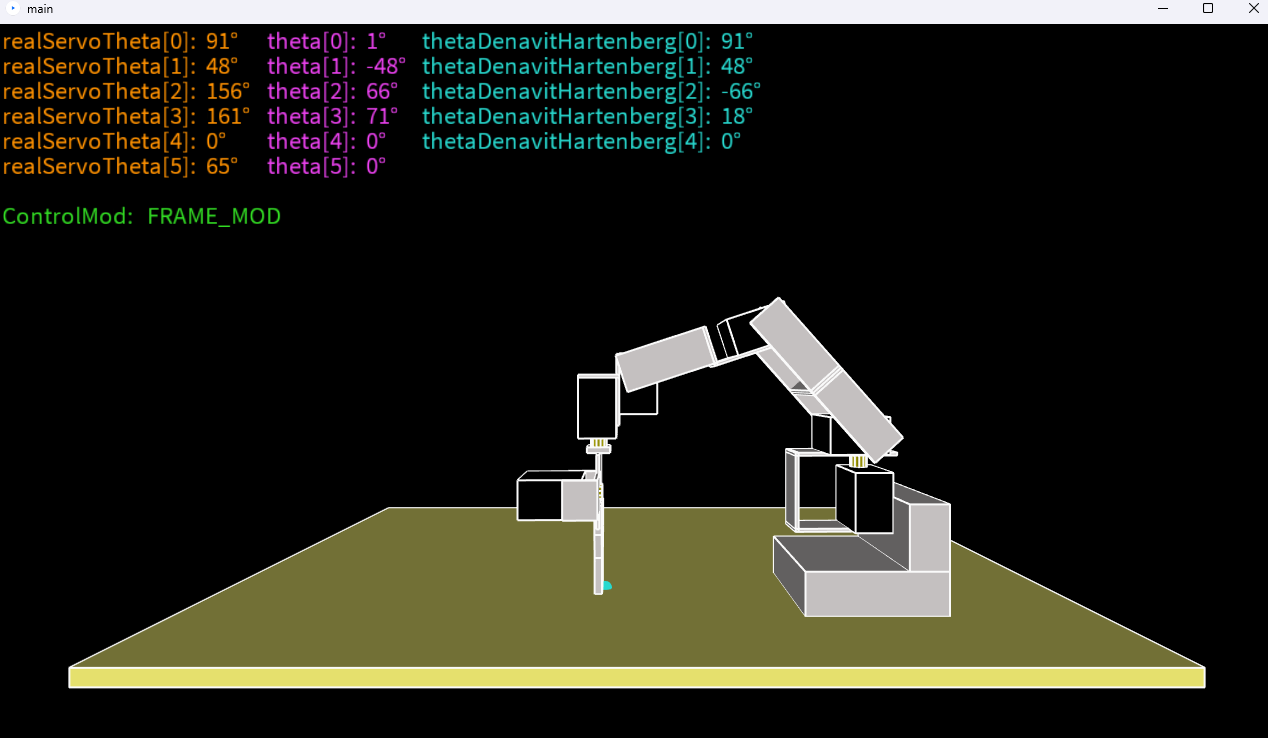
\includegraphics[width=15cm]{images/render3D.png}
    \end{figure}
    
    \subsection{Modalità e comandi}
    
    \begin{text}
        Il programma presenta tre modalità di funzionamento e ognuna di queste dispone di un set di comandi propri. Sono anche presenti comandi validi in tutte le modalità.
    \end{text}
    
    \subsubsection{Comadi base}
    
    \begin{text}
        In questa sezione vengono descritti i comandi comuni a tutte le tre modalità. Oltre ai comandi da tastiera è anche possibile premere con il maouse su un punto qualsiasi della finestra grafica per riposizionare il centro di rifermento del render 3D all'interno dello spazio di Processing.  \\ \\
        I comandi base(da tastiera) sono:
    \end{text}
    
    \begin{itemize}
      \item \textbf{tasto f/F:} arresta l'esecuzione del programma salvando su memoria di massa il contenuto dei file di log chiamati \textbf{connection\_data.txt} e \textbf{position\_data.txt}
      \item \textbf{tasto FRECCIA DESTRA:} ruota lo spazio 3D in senso antiorario rispetto all'asse verticale
      \item \textbf{tasto FRECCIA SINISTRA:} ruota lo spazio 3D in senso orario rispetto all'asse verticale
      \item \textbf{tasto FRECCIA ALTA:} sposta il render 3D in avanti verso l'utente
      \item \textbf{tasto FRECCIA BASSA:} sposta il render 3D in dietro verso l'utente
      \item \textbf{tasto 0:} ruota lo spazio 3D in senso orario rispetto all'asse orizzontale
      \item \textbf{tasto m/M:} permette di cambiare la modalità corrente, alternando fra le tre possibili
    \end{itemize}
    
    \subsubsection{Manual Mod}
    
    \begin{text}
        Questa è stata la prima modalità ad essere sviluppata, poiché la sua funzione era indispensabile per tarare correttamente le relazioni che intercorrono tra le diverse rappresentazioni degli angoli theta precedentemente descritti. \\ \\
        I comadi in \textbf{Manual Mod} sono:
    \end{text}
    
    \begin{itemize}
      \item \textbf{tasto q/Q:} resetta gli angoli theta al loro valore di default
      \item \textbf{tasto s/S:} cambia il verso di rotazione di tutti i motori
      \item \textbf{tasto 1:} aziona la rotazione del motore 1
      \item \textbf{tasto 2:} aziona la rotazione del motore 2
      \item \textbf{tasto 3:} aziona la rotazione del motore 3
      \item \textbf{tasto 4:} aziona la rotazione del motore 4
      \item \textbf{tasto 5:} aziona la rotazione del motore 5
      \item \textbf{tasto 6:} aziona la rotazione del motore 6
    \end{itemize}
    
    \subsubsection{Inverse Kinematic Mod}
    
    \begin{text}
        Questa modalità è quella che implementa il calcolo della cinematica inversa e che a sua volta si è resa indispensabile per poter successivamente realizare la terza modalità. \\ \\
        I comadi in \textbf{Inverse Kinematic Mod} sono:
    \end{text}
    
    \begin{itemize}
      \item \textbf{tasto g/G:} imposta il gomito alto o basso per il calcolo della cinematica inversa.
      \item \textbf{tasto q/Q:} decrementa il valore della coordinata X desiderata
      \item \textbf{tasto w/W:} incrementa il valore della coordinata X desiderata
      \item \textbf{tasto e/E:} decrementa il valore della coordinata Y desiderata
      \item \textbf{tasto r/R:} incrementa il valore della coordinata Y desiderata
      \item \textbf{tasto t/T:} decrementa il valore della coordinata Z desiderata
      \item \textbf{tasto y/Y:} incrementa il valore della coordinata Z desiderata
      \item \textbf{tasto u/U:} decrementa il valore dell'angolo $\beta$ desiderato
      \item \textbf{tasto i/I:} incrementa il valore dell'angolo $\beta$ desiderato
      \item \textbf{tasto o/O:} decrementa il valore dell'angolo $\omega$ desiderato
      \item \textbf{tasto p/P:} incrementa il valore dell'angolo $\omega$ desiderato
      \item \textbf{tasto a/A:} apre la pinza
      \item \textbf{tasto s/S:} chiude la pinza
    \end{itemize}
    
    \subsubsection{Frame Mod}
    
    \begin{text}
        Questa modalità è la più particolare nonché il risultato dello sviluppo delle precedenti modalità. Si occupa di comunicare alla scheda Arduino, in ogni istante di tempo, i valori dei singoli angoli che compomgono un frame. L'insieme dei frame costituisce un movimento complesso che il robot compie ripetutamente, esattamente come se fosse impiegato in un vero processo industriale. I frame sono memorizzati nel file \textbf{frames\_data.txt} che il programma legge al suo avvio. Il file è di grandi dimensioni ed è stato realizzato sfruttando l'Inverse Kinematic Mod per calcolare gli angoli corrispondenti al \textbf{movimento} studiato prendendo in considerazione la terna [$x_d$, $y_d$, $z_d$], gli angoli $\beta_d$, $\omega_d$ e la rotazione del motore addetto alla pinza. \\ \\
        Questa modalità non presenta comandi specifici associati ad essa, sono comunque sempre validi i comandi base del programma.
    \end{text}
    
    
    
    \section{Arduino}
    
    \begin{text}
        La scheda Arduino UNO svolge la funzione di driver per i servomotori, che movimentano i giunti e la pinza del robot. Inoltre pilota un display LCD 16x2 che mostra all'utente i valori correnti degli angoli attutati dai servomotori rispetto al loro proprio sistema di riferimato (chiamati \textbf{realServoTheta[i]} su Processing).
    \end{text}
    
    \subsection{Schema elettrico}
    
    \begin{text}
        Il circuito elettrico è costituito da un alimentatore da laboratorio in grado di erogare fino a 300W in corrente continua, 6 servomotori, 1 display LCD, cavi per i collegamenti, il microcontrollore Arduino UNO e 2 breadboard per la prototipazione. I servomotori sono controllati tramite segnali PWM, che la scheda Arduino UNO genera in base ai valori ricevuti tramite la comunicazione seriale con Processing.
    \end{text}
    
    \subsection{Codice Arduino}
    
    \begin{lstlisting}[style=myarduinostyle, caption=Parti principali del firmware]
        void setup() {
        
          Serial.begin(9600);
          lcd.begin(16, 2);  
          lcd.print("Hello Scorbot!");
          myRobot.setupRobot();
        
          pinMode(PIN_LED, OUTPUT);
          digitalWrite(PIN_LED, LOW);
        
          if (Serial.available() > 0) {  // pulisco il buffer della porta seriale
            while (Serial.read() != -1);
          }
        
          if (Serial.availableForWrite()) {
            Serial.write(ARDUINO_ID);
          }
        
          while (loop_flag) {
            if (Serial.available() >= strlen(PROCESSING_ID)) {
              id = Serial.readString();
        
              if (id.equals(PROCESSING_ID)) {
                digitalWrite(PIN_LED, HIGH);
                loop_flag = false;
              }
            }
          }
        
          point_ascii[0][3] = '\0';
          point_ascii[1][3] = '\0';
          point_ascii[2][3] = '\0';
          point_ascii[3][3] = '\0';
          point_ascii[4][3] = '\0';
          point_ascii[5][3] = '\0';
        }
        
        void loop() {
        
          if (Serial.available() >= strlen(PROCESSING_ID)+3*MOTORS_NUM) {
            Serial.readBytes(buffer, strlen(PROCESSING_ID));
            id = buffer;
            
            if (id.equals(PROCESSING_ID)) {
            
              for(i=0; i<MOTORS_NUM; i++) {
                Serial.readBytes(&point_ascii[i][0], 3);
              }
              
              pos.x1 = atoi(&point_ascii[0][0]);
              pos.x2 = atoi(&point_ascii[1][0]);
              pos.x3 = atoi(&point_ascii[2][0]);
              pos.x4 = atoi(&point_ascii[3][0]);
              pos.x5 = atoi(&point_ascii[4][0]);
              pos.x6 = atoi(&point_ascii[5][0]);
        
              lcd.clear();
              lcd.home();
        
              lcd.print(&point_ascii[0][0]);
              lcd.print("-");
              lcd.print(&point_ascii[1][0]);
              lcd.print("-");
              lcd.print(&point_ascii[2][0]);
        
              lcd.setCursor(0,1);
        
              lcd.print(&point_ascii[3][0]);
              lcd.print("-");
              lcd.print(&point_ascii[4][0]);
              lcd.print("-");
              lcd.print(&point_ascii[5][0]);
        
              myRobot.setPosition(&pos);
        
              if (Serial.availableForWrite()) {
                Serial.write(ARDUINO_ID);
              }
            }
          }
        }
    
    \end{lstlisting}
    
    \addcontentsline{toc}{section}{Bibliografia}
    
    
    
    \begin{thebibliography}{10}
    
        \bibitem{Denavit-Hartenberg}
            F. Martinelli, \emph{Denavit-Hartenberg, 11/10/2022}, dispense del corso di Robotica con Laboratorio, \url{http://robot2.disp.uniroma2.it/~fmartine/RobLab/appuntiLezioni/DenHart.pdf}
        
        \bibitem{Scorbot}
            F. Martinelli, \emph{Cinematica diretta e inversa del robot SCORBOT, 14 e 18/10/2022}, dispense del corso di Robotica con Laboratorio, \url{http://robot2.disp.uniroma2.it/~fmartine/RobLab/appuntiLezioni/SCORBOT.pdf}
        
        \bibitem{Elettronica}
            G. Ortolani, E. Venturi, \emph{Manuale di elettrotecnica, elettronica e automazione}, 2017, Hoepli.
    
        \bibitem{Processing}
            Documentazione ambiente di sviluppo Processing, \url{https://processing.org/reference}
    
        \bibitem{Arduino}
            Documentazione ambiente di sviluppo Arduino, \url{https://www.arduino.cc/reference/en/}
    
    \end{thebibliography}

\end{document}
